%!TEX root=../documentation-bachlorthesis-speicherarchitektur-lstucker.tex
\cleardoublepage
\chapter{Speicherarchitekturen}

Sowohl private Personen als auch Unternehmen haben unterschiedliche Anforderungen an die Speicherung ihrer Daten. Während früher die Daten in der Regel in einem integrierten Speicher des Computersystems verwaltet wurden, werden heute eine breite Paletten an Speicherlösungen am Markt angeboten. Ein Grund dafür ist der kontinuierlich wachsende Bedarf an mehr Speicherkapazität aber auch zusätzliche Anforderungen an die Verwaltung der Daten, die Datensicherung. Spezifische Daten zu suchen und zu bearbeiten soll heute einfach, effizient und zu günstigen Kosten möglich sein, was laufend neue Lösungsansätze bedingt und es nicht einfacher macht, auf das richtige Pferd bzw. Technologie zu setzen. Wer möchte morgen schon gezwungen sein, seine mühsam aufbereiteten Daten in einem aufwendigen Migrationsverfahren, womöglich mit einem notwendigen Datenverlust, in ein neues System zu übernehmen? Eine genauere Betrachtung des Angebotsmarktes für die vorhandenen und die künftigen sich durchzusetzenden Technologien drängt sich deshalb auf.

Die heutigen am Markt erhältlichen Speicherarchitekturen lassen sich in der obersten Kategorie in Block- (Block-based), Datei- (File-based) und Objekt- (Object-based) basierte adressierende Systeme unterteilen. Die Kategorien zur Einteilung der verschiedenen Lösungen lässt sich nicht exakt zuordnen, da einige Speicherlösungen aus einem Mix aus mehreren Kategorien bestehenden können.

\section{Block-basierend}
Die Block-basierende Speicherarchitektur ist wohl die traditionellste von allen und ist die am weitverbreiteste Form. Die meisten Computersysteme, sei es Server, Desktop-PCs, Tablet-PC, Smartphones, Spielkonsole, verwaltet ihre Daten in einem blockbasierenden Speicher. Als Speichermedium wird in diesen Geräten oft eine magnetische Festplatte, Solid State Disk oder ein Flash-Speicher verwendet.

Bei Block-Speicher werden Daten in Blöcke gelesen und gespeichert (adressiert), ein Block bildet sich aus einer Sequenz von Bits bzw. Bytes. Die Grösse eines Blocks wird als Blocklänge bezeichnet und ist bei allen Blöcken einer Einheit gleich gross. 

Experten wie Mike Mesnier, Greg Ganger und Erik Riedel, sehen jedoch bei zunehmender Speichergrösse und Komplexität von Systemen fundamentale Einschränkungen von Block-Schnittstellen.

\begin{quotation}
\em Since the first disk drive in 1956, disks have grown by over six orders of magnitude in density and over four orders in performance, yet the storage interface (i.e., blocks) has remained largely unchanged. Although the stability of the block-based interfaces of SCSI and ATA/IDE has benefited systems, it is now becoming a limiting factor for many storage architectures. As storage infrastructures increase in both, size and complexity, the functions that system designers want to perform are fundamentally limited by the block interface. \end{quotation}\cite{Mesnier2003}

Vergleicht man die Performance der ersten Festplatte, welche von IBM produziert wurde, mit einer heute erhältlichen Seagate Festplatte (Jahr 2011), so hat sich die Speicherdichte von 2000 bit per Quadratzoll auf 625 Gigabyte und die Transferrate von 8 Kilobyte auf 600 Megabyte pro Sekunde verbessert. \cite{Seagate2011}\cite{Seagate2011a}

Für den Zugriff auf blockbasierende Speichersysteme werden meist Schnittstellen-Protokolle wie das Small Computer System Interface (SCSI) oder Advanced Technology Attachment (\gls{ATA}) verwendet. Diese Protokolle wurden jedoch in einer Zeit entwickelt, als man davon ausging, dass ein Blockspeicher jeweils nur von einem Computersystem verwendet wird und nicht mit mehreren Computersystemen geteilt werden soll. Diese Annahme für single user systems stimmt für den Consumer Elektronic Bereich mehrheitlich noch heute. In Bereichen jedoch, in denen grosse Speicherkapazitäten oder eine hohe Verfügbarkeit für viele gleichzeitige Benutzer gefordert sind, wie dies viele Geschäftsanwendungen charakterisiert, stimmen diese Annahmen nicht mehr.

Für blockbasierende Speicher, welche nicht als Server-interne Speicher bestehen, unterscheidet man den Direct Attached Storage (DAS) und das Storage Area Network (SAN). 

\subsection{Direct Attached Storage}
Bei DAS handelt es sich, wie es aus der englischen Bezeichnung zu entnehmen ist, um Speicher, welcher direkt an ein Computersystem angeschlossen wird. Bei DAS Enclosure handelt sich um ein Gehäuse mit mehreren verbauten Festplatten, welche üblicherweise über einen Host-Bus-Adapter an ein Computersytem angeschlossen werden. Als Schnittstellen-Protokoll werden \gls{ATA}, \gls{SATA}, \gls{eSATA}, \gls{SCSI}, \gls{SAS} oder Fibre Channel eingesetzt. DAS können mit mehreren Computersystemen geteilt werden, sofern genügend Schnittstellen zur Verfügung stehen.

\subsection{Storage Area Network}
Die Storage Networking Industry Association (\gls{SNIA}) definiert ein Storage Area Network (SAN) als ein Netzwerk, dessen primärer Bestimmungszweck das Transferieren von Daten zwischen Computersysteme und Speicherelemente und unter Storage Elemente ist. Ein SAN besteht aus einer Kommunikations-Infrastruktur, welches eine physische Verbindung und eine Management-Schicht beinhaltet, das die Verbindungen, die Speichereinheiten und das Computersystem organisiert, damit der Datentransfer sicher und robust erfolgen kann. Der Begriff SAN wird normalerweise (aber nicht notwendigerweise) mit dem Block I/O Service in Verbindung gebracht und weniger mit dem Datei-Zugriff-Service. \cite{SNIA2011}

Je nach SAN Implementierung kommen folgende Geräte bzw. Komponenten vor:
\begin{itemize}
\item Server
\item Host Bus Adapter
\item Gigabit Interface Converter
\item SAN-Switch
\item Storage system (Speichersystem)
\item Tape Library
\item Logical Unit
\end{itemize}

\paragraph*{Server} 
Der Server greift über das SAN auf Ressourcen von Speichersystem oder Tape Library zu. In einzelnen Fällen kann der Server selbst über SAN anderen Servern Speicher zur Verfügung stellen.

\paragraph*{Host Bus Adapter}
Host Bus Adapter (HBA) für das SAN sind intelligente Hardwareschnittstellen, welche für die Verbindung von Server in einem SAN verwendet werden. Sofern die Server nicht bereits mit einem Host Bus Adapter ausgerüstet sind, können diese normalerweise durch Host Bus Adapter in form von Steckkarten erweitert werden. Der Host Bus Adapter selber hat pro Port einen Einschub, in welche ein Gigabit Interface Converter eingebaut wird. \cite{Christopher2009}

\paragraph*{Gigabit Interface Converter}
Der Gigabit Interface Converter ist eine modulare Schnittstelle, welche elektrische Signale in optische Signale umwandeln. \cite{SNIA2011}

\paragraph*{SAN-Switch}
Der SAN Switch ist ein Koppler, welcher dezidiert für die SAN-Umgebung verwendet wird.

\paragraph*{Speichersystem}
Das Speichersystem stellt im SAN den geteilten Speicher zur Verfügung. Gemäss den IT Marktforschung und Analyse Unternehmen Gartner gehören \gls{EMC}, \gls{IBM}, NetApp, \gls{Dell}, \gls{HP}, \gls{HitachiDataSystems} zu den Marktführern. \cite{RogerW.CoxPushanRinnenStanleyZaffos2011}

\paragraph*{Tape Library}
Tape Library ist eine Bandbibliothek, in welchem sich ein oder mehrere Bandlaufwerke und mehrere Magnetbänder befinden und meistens der automatische Bandwechsel mittels eines Bandroboters realisiert wird. Das Tape Library wird für die Sicherung von Daten auf Band eingesetzt.

\paragraph*{Logical Unit}
Ein Logical Unit ist ein Gerät, welches über SCSI-Protokoll über das Logical Unit Number (LUN) andressiert wird. Das Gerät wird, technisch nicht korrekt, oft als LUN bezeichnet. Im Speichersystem werden z.B. mehrere Festplatten mittels RAID zu einer Einheit zusammengefasst. Sofern keine weitere Virtualisierung von dem Speicherhersteller zum Einsatz kommt, wird die zusammengefasste Einheit wiederum in Speichereinheiten aufgeteilt und diese als LUN dem Server zugeteilt. \cite{SNIA2011}

\subsubsection{Fibre Channel}
SCSI ist zwar sehr populär, ist jedoch mit 80 Mbps Geschwindigkeit, mit maximal 25 Meter Buslänge und mit maximal 32 Geräten pro Bus, ein limitierender Faktor für viele Anwendungen. Unter anderem wegen den erwähnten Limitierungen von SCSI hat das American National Standards Institute (ANSI) die Fibre Channel Technik entwickelt. Fibre Channel ist ein mehrschichtiges Netzwerk, welches die charakteristischen Funktionen für die Übertragung von Daten über ein Netzwerk definiert. Der Standard enthält von der physikalischen Schnittstelle, Daten Codierung, Übertragungssteuerung (Link Control), Fluss Kontrolle, bis hinzu den Protokoll Schnittstellen. Im Vergleich zu anderen Netzwerken beinhaltet die Fibre Channel Architektur einen signifikanten Anteil von Hardware Prozessen, um eine hohe Performance zu erreichen. \cite{Gupta2002}\cite{Christopher2009}

Beim Design von Fibre Channel hat man darauf geachtet, die besten charakteristischen Eigenschaften der I/O Bus-Kommunikation (Channel) zwischen zwei Geräten und der Netzwerk- Kommunikation zwischen mehreren Geräten zu kombinieren. Die Channel-Kommunikation ist im Vergleich zur Netzwerk-Kommunikation, hardwareintensive, schnell und produziert wenig Overhead. Netzwerk-Kommunikation ist hingegen abhängig von der Softwareimplementierung, das Protokoll, unterstützt aber die Kommunikation für eine grosse Anzahl von Geräten.

Anders als es der Namen von Fibre-Channel vermuten lässt, ist Fibre-Channel nicht auf Fiberoptik-Kabel als Träger-Medium beschränkt, sondern lässt sich ebenso mit Kupferkabel betreiben. Aufgrund von physikalischen Eigenschaften ist das Fiberoptik-Kabel gegenüber dem Kupferkabel in Geschwindigkeit kombiniert mit Distanz überlegen. So liegt die maximale Distanz bei Kupferkabel bei 30 Metern bei einer Geschwindigkeit von 1 Gbps, bei höheren Geschwindigkeiten wird die maximale Distanz noch weiter reduziert. Beim Fiberoptic-Kabel wird die maximale Distanz der Signalübertragung von der Installationsqualität, des Fiberoptic-Kabeltyps, des Kern-Durchmessers, der Lichtwellenlänge Rundreise Latenz und der eingesetzter Hardware bestimmt. Je weiter das Licht innerhalb des Kabels übertragen werden muss, desto grösser ist der Verlust der ursprünglichen Signalstärke. Mit spezieller Hardware können auch Distanzen von bis zu 600 Kilometer \footnote{\url{http://www.enterprisestorageforum.com/industrynews/article.php/2171801/Synchronous-SAN-Sets-Fibre-Channel-Distance-Record.htm}} erreicht werden.

Es gibt drei Fibre Channel Topologien:
\begin{itemize}
\item Point-to-Point
\item Arbitrated-Loop
\item Switched-Fabric
\end{itemize}

\paragraph*{Point-to-Point-Topologie}
Die Point-to-Point-Topologie ist die direkte Verbindung von zwei Fibre Channel Geräten. Oft handelt es sich um eine Verbindung von einem Server und einem Speichersystem, wie dies im Direct Attached Storage (DAS) Umfeld vorkommt. \cite{Christopher2009}

\paragraph*{Arbitrated-Loop-Topologie}
Bei der Arbitrated-Loop-Topologie können bis zu 126 Knoten (NL\_Ports) in einem geteilten Bus-Ring zusammengeschlossen werden. In diesem Ring kann eine Verbindung zwischen zwei Ports aktiv sein, während alle anderen Ports als Repeater arbeiten und das Signal weiterleiten. Die Arbitrated-Loop-Topologie ist in seiner Architektur dem Token-Ring ähnlich. \cite{Gupta2002}\cite{Christopher2009}

\paragraph*{Switched-Fabric-Topologie}
Die klassische SAN Topologie basiert auf der Switched-Fabric-Topologie. Eine Switched-Fabric-Topologie besteht aus einer oder mehreren Switches, die zu einer Fibre-Channel-Fabric zusammengeschlossen werden. Die einzelnen involvierten FC-Geräte, wie Server oder Storagesysteme, werden über eine oder mehrere Ports an eine Switched-Fabric angeschlossen. In einer Fabric können bis zu $2^{24}$ Ports angeschlossen werden. \cite{Gupta2002}\cite{Christopher2009}

Mit der Switched-Fabic-Topologie lassen sich verschiedene Fabric Topologien bilden.
Die einfachste Topologie, welche die Eliminierung von "'Single Point of Failure"' zum Ziele hat, ist die Dual Switch Topologie, wie in der \refabb{abb:DualSwitchTopologie} dargestellt. In dieser Topologie dient jeder Switch als eigenständige Fabric. Die FC-Geräte wie Server und Storagesysteme werden jeweils pro Fabric bzw. Switch mit mindestens einem FC-Port angeschlossen. Durch den Einsatz von Path Management Software auf dem Server, kann eine vom Speichersystem zugeteilte Logical Unit über mehrere Path angesprochen werden. Diese Implementierung bietet gleich verschiedene Vorteile. Wenn ein Path oder eine ganze Fabric ausfallen sollte, übernimmt der andere Path automatisch die Kommunikation. Bei Wartungsarbeiten an Komponenten einer Fabric kann der Service ohne Downtime des Gesamtsystems weiter betrieben werden. Moderne Path Management Software und Speichersysteme unterstützen zudem die Lastverteilung (Loadbalance) der I/O-Last über alle Paths. \cite{Christopher2009}

\begin{center}
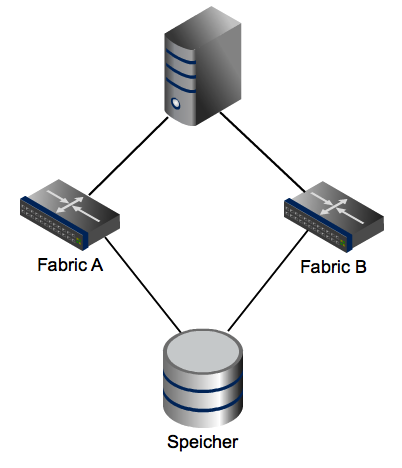
\includegraphics[width=\linewidth, keepaspectratio = true]{media/dualSwitchTopologie.png}
\mycaption{figure}{\label{abb:DualSwitchTopologie}Fibre Channel SAN mit Dual Switch Topologie}
\end{center}

Die Meshed Fabric Topologie erhöht die zusätzlich die Ausfallsicherheit innerhalb einer einzelnen Fabric. Für die Meshed Fabric sind pro Fabric mindestens vier Fibre Channel SAN Switches erforderlich. Jeder Switch wird, wie in \refabb{abb:MashedFabricTopologie} ersichtlich, mit mindestens einem Path, den sogenannten Inter-Switch-Link (ISL), zu allen anderen Switches in der Fabric verbunden. Die Meshed Fabric kann den gleichzeitigen Ausfall von mehreren Kabeln und Switches verkraften, ohne dass deshalb die ganze Fabric ausfällt. \cite{Christopher2009}

\begin{center}
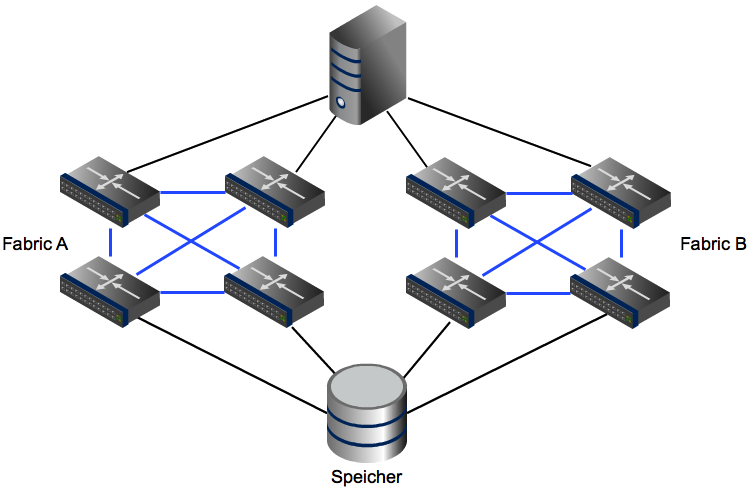
\includegraphics[width=\linewidth, keepaspectratio = true]{media/MashedFabric.png}
\mycaption{figure}{\label{abb:MashedFabricTopologie}Fibre Channel SAN mit Mashed Fabric Topologie}
\end{center}

\subsubsection{iSCSI}
Das SCSI-Protokoll ist ein populäres Protokoll für die Kommunikation mit I/O Geräten speziell für Speichergeräte. SCSI weist die Client-Server Architektur auf, wobei die Clients bei SCSI Interfaces als "initiators" bezeichnet werden und die logische Einheit vom Server als "target".

SCSI Protokoll wurde schon über Protokolle transportiert, jedoch waren all die Transportprotokolle in der Distanz limitiert. \gls{IBM} startete 1996 mit der Forschung für die Übertragung von SCSI über das Ethernet, dabei untersuchte \gls{IBM}, ob sich der Transport mittels IP oder \gls{TCPIP} besser eignen würde. Messungen zeigten damals, dass in einem lokalen Netzwerk der Transport mittels IP besser als \gls{TCPIP} geeignet ist. Mit den erwarteten künftigen Entwicklungen bezüglich des Datentransports über die lokalen Netzwerkgrenzen hinaus war hingegen der Einsatz von TCP/IP die bessere Wahl. 1999 hatten sich \gls{IBM} und \gls{Cisco} darauf geeinigt, "SCSI over TCP/IP" gemeinsam in einer Internet Engineering Task Force (\gls{IETF}) als Industriestandard weiterzuentwickeln \cite{JohnL.202}. Die definitive Spezifikation von SCSI over \gls{TCPIP} ist im \gls{RFC} 3720 mit dem Namen iSCSI im April 2004 fertiggestellt worden. \cite{J.Satran2004}

% \paragraph*{Kosten}
Für den Betrieb eines Fibre Channel SAN sind spezielle Hardware und Fibre Channel Kenntnisse notwenig. Da bei iSCSI dieselbe Technik wie im Computernetzwerk verwendet wird, benötigt der Aufbau und Betrieb von Netzwerk Infrastruktur und Management Software Lösungen keine zusätzliche Ausbildung, was die Gesamtbetriebskosten (TCO) substanziell senkt.

Grundsätzlich kann jeder Computer, welcher mit einem Netzwerkanschluss ausgerüstet ist und einen iSCSI Software Treiber hat, iSCSI nutzen. Computer, welche genügende Prozessorleistung aufweisen, können die zusätzliche Last für die Verarbeitung von iSCSI mit konventionellen Netzwerkkarten lösen. Computersysteme für welche die Verarbeitungsgeschwindigkeit kritisch ist, kann diese zusätzliche Last eine Bürde sein. Vergleichbar wie bei Fibre Channel gibt es für iSCSI spezielle Netzwerkkarten bzw. Host Bus Adapter, welche mittels TCP/IP Offload Engine (TOE) und volle iSCSI Offload Engine im eigenen Chip die \gls{TCPIP} bzw. iSCSI Pakete verarbeiten. Solche Netzwerkkarten entlasten die Central Processing Unit (\gls{CPU}) des Servers wesentlich und weisen bessere Werte in der Latenz auf.

% \paragraph*{Netzwerk}
In einem Ethernet Netzwerk verwaltet sich jeder Switch mehr oder weniger autonom und führt eine eigene Weiterleitungstabelle, mit welcher der Switch entscheidet, über welchen Port ein Ethernet Paket ausgeliefert werden muss. Dazu enthält die Weiterleitungstabelle pro MAC Adresse den dazugehörigen Port. Trifft ein Ethernet Paket mit noch unbekannter MAC Adresse ein, leitet der Switch das Paket über alle Ports weiter. Durch die Rückantwort vom Zielsystem lernt der Switch, über welchen Port dieses erreichbar ist. Werden in einem Switch Netzwerk benachbarte Switches untereinander über mehrere Pfade verbunden, kann es in einem solchen Szenario vorkommen, dass das Paket wieder am ursprünglichen Switch ankommt, wenn der benachbarte Switch die MAC-Adresse ebenfalls nicht kennt. Es entsteht dadurch eine Verdoppelung des Ethernet Paketes im Netzwerk bzw. es kommt zu einer Schleifenbildung, was in der Folge zu einer Netzwerkstörung führt. Mittels Spanning Tree Protokoll (STP) sollen solche Schleifen vermieden werden. Das Spanning Tree Protokoll erstellt eine Baum Topologie mit jeweils einem aktiven Path zwischen zwei Switches. Diese Topologie hat verschiedene Nachteile: 

\begin{itemize}
\item Beim Topologie-Wechsel wird im Netzwerk der Spanning Tree neu ausgehandelt. Während dieser Neuaushandlung ist der Datentransport während mindestens 15 Sekunden unterbrochen. Ein typischer Topologiewechsel kann zum Beispiel durch einen Pfad-Ausfall zwischen zwei Switches hervorgerufen werden.

\item In einer Baum-Hierarchie müssen die Pakete innerhalb des Baumes der Hierarchie entsprechend weitergeleitet werden (auf und ab) und können nicht über einen theoretisch direkteren Pfad quer weitergeleitet werden. Befindet sich z.B das Ziel auf der anderen Baumseite, muss das Paket die ganze Hierarchie hinauf und auf der anderen Seite hinunter bis zum Zielsystem weitergeleitet werden. Könnten die Switches über mehrere Pfade miteinander kommunizieren, so würde dem Datentransport über den direkten Weg nichts im Wege stehen und würde zudem weniger Switches involvieren bzw. belasten.
\end{itemize}

Hersteller wie Brocade haben diese Problematik für den Betrieb von iSCSI SAN erkannt und haben Lösungen entwickelt, welche das Prinzip von Fibre Channel Fabrics für Ethernet Netzwerke umsetzen. Bislang ist dafür noch kein allgemein verbindlicher Standard entstanden und proprietäre Lösungen sich im Markt kaum durchsetzen können.

%\paragraph*{Sicherheit}
Wie beim Fibre Channel SAN sollte im Geschäftsumfeld iSCSI über ein dediziertes Netzwerk laufen. Die Abgrenzung erhöht die Sicherheit einerseits und das Storage Netzwerk ist andererseits klar von anderen Netzwerken abgeschottet. Fehlerhafte Firewall-Regeln für das Computer Netzwerk haben keinen direkten Einfluss auf die Sicherheit des Datennetzwerkes. Störungen oder Überlast im Computer Netzwerk beeinflussen nicht die iSCSI Verbindungen. Mittels IPsec kann die Sicherheit durch die verbesserte Authentifizierung und der optionaler Verbindungsverschlüsselung weiter erhöht werden. 

%\paragraph*{Integrität}
iSCSI stellt die Integrität des übermittelten Paketes mit dem CRC-32c Digests sicher. 

\paragraph*{Skalierbarkeit Datenvolumen}
Einem Server können mehrere Logical Units zugeteilt werden. Durch den Einsatz eines Volume Managers können mehrere Logical Units zu einer grossen logischen Volume zusammengefasst werden. Sollte die Kapazität eines Speichersystems nicht ausreichen, kann ein weiteres Speichersystem an das SAN angeschlossen werden.

\paragraph*{Durchsatz I/O}
Die Firma Netapp zählt zu den Marktführern für unternehmensweite NAS Speicherlösungen. Neben dem "Network File System" (NFS), unterstützen die Speicherlösungen von Netapp auch die Integration von Logical Units über iSCSI als auch über Fibre Channel. Saad Jafri und Chris Lemmons von Netapp haben die Bereitstellung von Speichern über die verschiedenen Verfahren bezüglich Performance für eine VMWare vSphere Umgebung untersucht. Netapp weisst in ihrem Report nicht die konkreten Messwerte aus, sondern lediglich die Werte im Vergleich zu einem 4Gb Fibre Channel.

Wie im \refabb{abb:NetappIOPS} von Netapp zu entnehmen ist, sind die I/O pro Sekunden Werte von iSCSI in einen 1Gb Ethernet Netzwerk im Vergleich zu dem 4Gb Fibre Channel rund 8\%tiefer. Wobei höhere Werte bei I/0 pro Sekunden besser sind. Im 10 Gb Ethernet Netzwerk erreicht iSCSI dieselben Werte wie Fibre Channel in einem 8Gb Netzwerk. \cite{Jafri2011}

\begin{center}
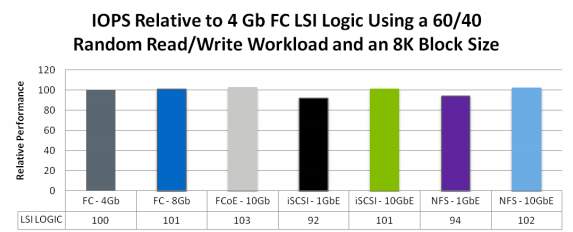
\includegraphics[width=\linewidth, keepaspectratio = true]{media/netapp_iops.png}
\mycaption{figure}{\label{abb:NetappIOPS}Netapp IOPS Durchsatz für alle unterstützten Protokolle im Vergleich zu 4Gb FC mit 8K Blockgrösse\cite{Jafri2011}}
\end{center}

Der Report von Netapp hat ebenfalls die Latenz verglichen. Bei der Latenz möchte man einen möglichst tiefen Wert erreichen. Gemäss \refabb{abb:NetappLatenz} ist die Latenz von iSCSI in einen 1 Gb Ethernet Netzwerk rund 9\% höher als bei Fibre Channel in einem 4Gb Netzwerk. Bei iSCSI in 10Gb Ethernet waren die Werte gleich gut wie Fibre Channel im 4Gb Netzwerk. Das Fibre Channel in einem 8Gb Netzwerk hatte jedoch rund 1\% tiefere Werte.\cite{Jafri2011}

\begin{center}
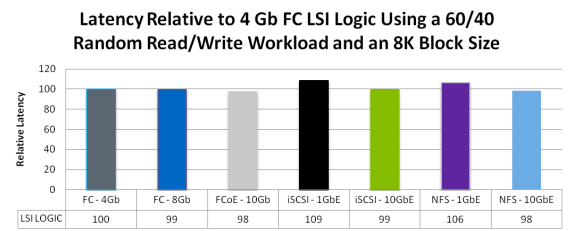
\includegraphics[width=\linewidth, keepaspectratio = true]{media/netapp_latence.png}
\mycaption{figure}{\label{abb:NetappLatenz}Netapp Latenz für alle unterstützten Protokolle im Vergleich zu 4Gb FC mit 8K Blockgrösse \cite{Jafri2011}}
\end{center}
 
\subsection{Logical Volume Manager}
Logical Volume Manager oder Dateisysteme, welche die Logik eines Logical Volume Managers kombinieren, ermöglichen mehrere Block-Geräte bzw. Logical Units zu einer grossen logischen Volume zusammenzufassen. Dies birgt den Vorteil, dass die maximale Grösse eines Block-Gerätes nicht der limitierende Faktor des darauf installierten Dateisystems ist. Neben dem Erstellen von Logischen Volumes können einige Logical Volume Manager den Last-Zugriff auf die verschiedenen Block-Geräte durch Striping optimaler verteilen und sorgen damit für eine besser Performance beim Datenzugriff. Eine weitere Aufgabe des Logical Volume Managers ist die redundante Haltung der Daten durch Spiegelung. Mittels serverseitiger Spiegelung (Host-Based Mirroring) können die Daten von zwei Standorten zur Verfügung gestellt werden. Dazu werden von zwei Speichersystemen, welche an unterschiedlichen Standorten installiert sind, gleich viele und gleich grosse Logical Units über das SAN dem Computersystem zugeteilt.

Klassische Server Linux Distributoren, wie Red Hat, Suse und Debian inkl. Ubuntu liefern den quelloffenen Logical Volume Manager 2 (LVM2) in ihrem Distributionspacket mit. Der LVM2 kann theoretisch auf einem 64-Bit System eine Logical Volume von 8 Exabyte bilden und adressieren. \cite{Levine2009}

Das ursprünglich von Oracle als ZFS-Ersatz entwickelte Btrfs Dateisystem könnte sich künftig zum Standard Dateisystem für viele Linux Server Distributionen mausern. Das für Solaris entwickelte ZFS als auch Btrfs kombinieren Dateisystem und Logical Volume Manager. Btrfs selbst wurde jedoch noch nicht als stabile Version veröffentlicht und ist deshalb für den produktiven Betrieb noch nicht empfehlenswert. \cite{Redler2011}


\subsection{Datei System}
Betriebssysteme adressieren die Daten auf Block-Geräten nicht direkt an, sondern greifen über das darüberliegende Dateisystem zu. Das Dateisystem organisiert wie und wo Dateien auf den Block-Geräten abgelegt werden und verwalten die freie Speicherkapazität. Einige Dateisysteme regeln auch die Zugriffsberechtigungen auf die Daten. Die Block-Geräte (Logical Units) können im SAN oder DAS an verschiedene Computersysteme gleichzeitig zugeteilt werden. Es ist die Aufgabe des Dateisystems sicherzustellen, dass mehrere Computersysteme gleichzeitig vom gleichen Dateisystem lesen bzw. auf dieses schreiben können. Konventionelle Dateisysteme wie Ext3 unter Linux gehen von einer exklusiven Nutzung des Speichers aus. Dieses Dateisystem enthält keine Funktionen, die den gleichzeitigen Zugriff auf Daten regeln. Problematik beim gleichzeitigen Zugriff ist die Sicherstellung der Datenkonsistenz. Schreiben zum Beispiel zwei Computersysteme gleichzeitig in dieselbe Datei, ist zu regeln, welche Änderung gültig ist, um Dateninkonsistenz zu vermeiden. Dateisysteme, welche den gleichzeitigen Datenzugriff erlauben, regeln den Zugriff auf Dateien z.B. mit einem Sperrmechanismus (locking). Schreibt ein Computersystem in eine solche gleichzeitig benutzte Datei, wird die Datei für Änderungen durch das andere Computersystemen gesperrt. Dieser muss sich den neuen aktuellen Stand mit einem Daten-Refresh wieder holen. Cluster Dateisysteme wie Red Hat Global Filesystem (GFS) und Red Hat Global Filesystem 2 (GFS2) unterstützen dieses Sperren. Das Dateisystem Red Hat GFS Version 2 unterstützt bei einem 64-bit-System theoretisch Dateisysteme bis 8 Exabyte, Red Hat gewährleistet jedoch nur einen Support von maximal 100 Terabyte. \cite{Levine2011}

Dateisysteme wie ZFS und Btrfs stellen die Integrität der Daten vor Veränderung, wie dies zum Beispiel durch einen Bit-Fehler auf dem Block Gerät oder im Memory entstehen könnte, mittels Prüfsumme sicher. Dabei wir zur jeder Datei eine Hash-Prüfsumme abgespeichert. Wird die Datei gelesen, wird die Prüfsumme aus der Datei neu berechnet und mit der abgespeicherten Prüfsumme verglichen. Sofern das Dateisystem ebenfalls gespiegelt ist, korrigiert das Dateisystem die fehlerhafte Datei aus der intakten Kopie automatisch. Dieses Verfahren wird auch als selbstheilend (self-healing) bezeichnet. \cite{Bonwick2005}\cite{Oracle}

Dateisysteme können mittels Sicherungssoftware auf Bandlaufwerke oder andere Speichermedien gesichert werden.


\section{Datei-Basierend}
Bei Datei-basierten Speicherarchitekturen werden Daten nicht wie bei Block-basierten Speicherarchitekturen über Blocke adressiert, sondern über Dateien.

Mit dem Aufkommen von Desktop-Computern, wurde die Rechenlast des zentralen Mainframecmputer wesentlich entlastet (verteilte Rechenlast auf viele kleine Rechner). Ohne die Vernetzung der Desktop-Computer mussten die Daten mittels portablen Speichermedien ausgetauscht werden. Dies mag in kleinen Umgebungen noch praktikabel gewesen zu sein, wurde jedoch mit der steigenden Anzahl der Teilnehmer zusehends schwieriger bis unmöglich. Verfügbarkeit und Konsistenz der Daten konnte nicht zufriedenstellend gelöst werden. Die direkte Vernetzung der Desktop-Computer erlaubte zwar den effizienten Datenaustausch über das Netzwerk, bot aber trotzdem keine gefällige Lösung für die Datenkonsistenz und Datensicherung. Die bessere Lösung war der gemeinsame zentral angelegte Speicher, in welchem sämtliche Unternehmensdaten für alle Benutzer verfügbar gehalten und mit einem regelmässigen Backup gesichert wurden. Alle Anwender verfügten immer über die aktuellste Version der Daten. Unternehmen wie Sun Microsystem, IBM, Microsoft und Apple erkannten die Bedürfnisse der Benutzer und entwickelten für ihre Betriebsysteme die Funktionen für den geteilten Datenzugriff.

Zu den bekanntesten und weitverbreitesten Lösungen zählen NFS und \gls{CIFS} (SMB).


\subsection{Network File System}
Das ursprünglich rein von der Firma SUN Microsystems (heute Oracle) 1984 entwickeltes Network-File-System, ermöglicht den gemeinsamen Zugriff von mehreren Computersystemen auf das Dateisystem eines zentralen Host (Server), als ob der einzelne Benutzer Zugriff auf ein lokales Dateisystem hat. Die zweite Version von NFS erschien 1989 und war die erste Version welche von Internet Standard Request for Comments (\gls{RFC}) standardisiert wurde und unter der \gls{RFC} Nummer 1094 \footnote{\url{http://tools.ietf.org/html/rfc1094}} veröffentlicht wurde. Für den Transport des NFS Protokolls wurde bis Version zwei ausschliesslich das \gls{UDP} Transportprotokoll unterstützt.
Die Version 3 von NFS (\gls{RFC} 1813)\footnote{\url{http://tools.ietf.org/html/rfc1813}}, die 1995 veröffentlicht wurde, war die erste Version, in der Computer, Betriebsystem, Netzwerk-Architektur und Transport-Protokoll unabhängig ist. Die Unabhängigkeit wird mit der Verwendung von Remote Procedure Call (\gls{RPC}) erreicht, welches wiederum ein eXternal Data Representation (\gls{XDR}) verwendet. \cite{Stern2001}

\begin{center}
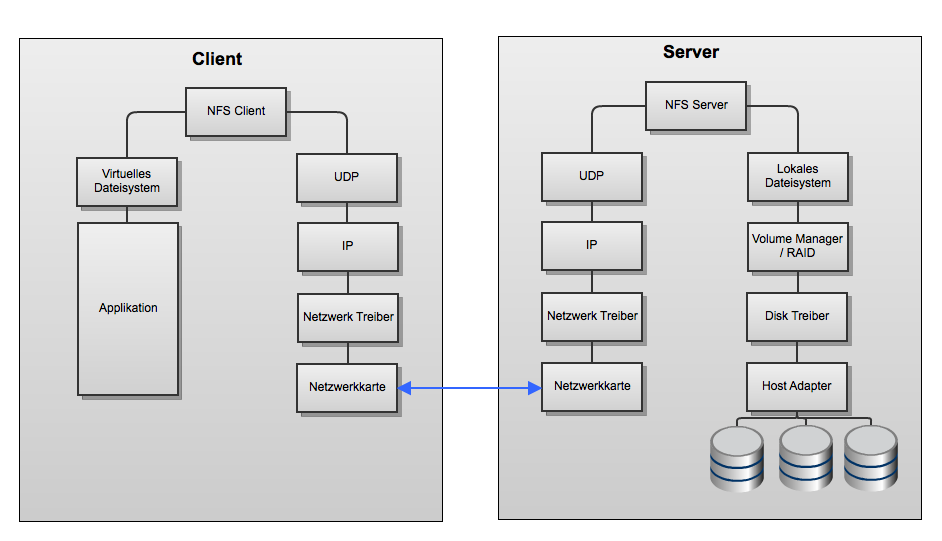
\includegraphics[width=\linewidth, keepaspectratio = true]{media/NFS.png}
\mycaption{figure}{\label{abb:NFSArchitektur}NFS Architektur \cite{Jafri2011}}
\end{center}

Wie im \refabb{abb:NFSArchitektur} zu entnehmen ist, ist NFS eine weitere Schicht, welche auf dem Dateisystem und dessen Block-Geräten des Computersystems bzw. Speichersystem aufbaut. So ist es zum Beispiel die Aufgabe des Dateisystems bzw. des Block-Gerätes, die Redundanz und Integrität der gespeicherten Daten sicherzustellen. 

Die Datenkonsistenz für den gleichzeitigen Zugriff von mehreren Computern stellt NFS mit einem separaten Protokoll, dem Network-Lock-Manager (NLM) sicher. Der Network-Lock-Manager sorgt dafür, dass eine Datei, welche von einem Computersystem geändert wird, vor der Änderung durch andere Benutzer, gesichert ist. Wenn ein Client eine Sperrung angefordert hat, muss derselbe Client dem Server die Entsperrung mitteilen, nachdem er die Daten nicht mehr benötigt. Diese Sperrlogik führt jedoch zu Problemen, wenn der Client vor der Entsperrung ein Systemabsturz erleidet, also die Entsperrung gar nicht mehr melden kann und somit die Datei für alle anderen Benutzer gesperrt bleibt.
NFS setzt mit NLM das Advisory Locking Sperr-Verfahren ein. Das bedeutet, dass andere Clients beim Zugriff auf eine gesperrte Datei nur darauf hingewiesen werden, dass die Datei gesperrt ist, ohne den Client daran zu hindern, eine gewünschte Änderung an den Daten vorzunehmen. \cite{Stern2001}

Seit Version 4 von NFS Protokoll (\gls{RFC} 3530) ist das Sperrverfahren (Locking) im Protokoll selber implementiert. Dadurch entfällt der zusätzliche Einsatz des Network Lock Managers. NFS Version 4 unterstützt zudem das Sperren eines Bytes-Bereiches innerhalb einer Datei. Der Client erhält vom Server lediglich einen Leasing-Zeitraum für die Sperrung (Lock), welche der Client vor Ablauf der Frist wieder erneuern muss, um sie aufrechtzuerhalten. NFS in der Version 4 erlaubt ferner das Sperrverfahren Mandatory Locking, das allen anderen Clients nicht ermöglicht, sich über die Sperrung hinwegzusetzen. \cite{Callaghan2003}

Indem NFS auf TCP/IP als Kommunikationsprotokoll aufbaut, kann eine NFS Freigabe, Standort übergreifend festgelegt werden. Es gilt auch hier, dass die Latenz und die Bandbreite der Verbindung zwischen den Standorten entscheidend ist und limitierend wirken kann.

NFS selbst hat keine eigene Implementierung für die Sicherstellung der Datenintegrität. Stattdessen verlässt sich NFS seit Version 2 auf die TCP und Ethernet Fehlererkennung. TCP prüft im Standardverfahren die Integrität mit einer 16-Bit-Integer Prüfsumme. Die 16-Bit-Integer Prüfsumme erkennt Fehler im pseudo IP-Header, TCP-Header und Daten. Das Verfahren zeigt Schwächen bei einzel Bit-Fehlererkennung. Ethernet verwendet für die Fehlererkennung eine CRC32 Prüfsumme. Diese ist zwar effektiv in der Erkennung und Behebung von Bit-Fehlern, bietet aber keinen durchgehenden (End-to-End) Schutz. Grund dafür ist beim Wechseln der Kollisionsdomäne-Paketes, wie es bei einen Swtich oder Router der Fall ist, da jedes Mal eine neu CRC32 Prüfsumme erstellt wird. Bei NFS ab Version 4 kann der Datentransfer zusätzlich mit Kerberos abgesichert werden. Kerberos hat einen strengen Schutz gegen Manipulationen am Datenpaket und stellt somit die Integrität der Daten sicher. Nachteilig ist nur, dass Kerberos zusätzlich eingerichtet werden muss. \cite{JohnL.202}

Bis und mit Version 4 war die Verarbeitung der Metadaten und die Verarbeitung der Daten in einem Protokoll und Server implementiert. NFS skalierte deshalb bei der Verarbeitung von Dateien mit grossem Speicherplatzbedarf nicht ausreichend. Fragt ein NFS-Client einen NFS-Server für eine Datei an, prüft der Server die Metadaten. Die Metadaten geben Auskunft über den Speicherort, die Grösse, das Erstellungsdatum und das Änderungsdatum einer Datei und wandelt die Anfrage in einen Disk I/O um. Die Daten der Datei werden gesammelt und über das Netzwerk übertragen. Bei kleinen Dateien benötigt der Server den grössten Zeitanteil für das Sammeln der Daten, während bei grossen Dateien der Transfer der Daten über das Netzwerk selbst der limitierende Faktor ist.
Mit der Entwicklung von pNFS konnte der Transfer der Daten parallelisiert werden. Die Architektur von NFS wurde dazu in mehrere Komponenten aufgeteilt. Der NFS Server besteht neu aus einem getrennten Metadaten Server und einem oder mehreren Daten-Servern. Die Aufgabe des Metadatenservers besteht darin, Ort und Art der Datenspeicherung zu verwalten. Die Daten-Server hingegen kümmern sich um Lese- und Schreibanfragen von den Clients.
Bei einer Anfrage für eine grosse Datei können mehrere Daten-Server parallel Teile der Datei dem Client ausliefern. Der Client kann dann die verschiedenen Teile wieder zu einer ganzen Datei zusammensetzen. \cite{Shepler2010}\cite{Group2010}

Mit der NFS Version 4.1 wurde pNFS Bestandteil von NFS und ist seit 2010 im \gls{RFC} 5661 standardisiert. Server Linux Distributoren, wie Red Hat haben vorerst NFS 4.1, erst als Vorschau in ihre Distribution integriert. \cite{EastJacquelynnMichaelHidep-Smith2011}




\subsection{NAS Appliance}

Network Attached Storage (NAS) sind Speichersysteme mit einem angepassten Dateisystem für den gemeinsamen Dateizugriff in einer heterogenen Computer Netzwerkumgebung, welche über ein LAN angeschlossen sind. Als Speicher verwenden NAS je nach Typ interne Festplatten, Direct Attached Storage oder einen über SAN angefügten Speicher.
An Clients stellen NAS den Speicher über NFS, CIFS, ISCSI zur Verfügung. High-End NAS können den Speicher auch über Fibre-Channel zur Verfügung stellen.

Gemäss Gartner gehören die Anbieter \gls{IBM}, \gls{EMC} und NetAPP zu den führenden NAS Anbietern im Midrange und High-End-Bereich. Gemäss Garnter gehört Magic Quadrant Netapp zusammen mit EMC zu den innovativsten Anbietern.

\begin{quotation}
\em 
\textbf{Strengths}
\begin{itemize}
\item NetApp remains one of the few truly unified storage providers among all top-tier vendors, with its software features continuing to be industry benchmarks. The company was able to regain some of the NAS revenue market share that it had lost in 2009. Its fast revenue growth in 2010 was driven by its successful campaign targeted at midsize enterprises with the value propositions of NFS supporting VMware and unified storage in consolidating Windows application storage.

\item In 2010, NetApp increased its aggregate up to 100TB with Data ONTAP 8.0.1 and introduced compression to complement its popular deduplication capability. It added a RESTful object storage interface (based on its acquisition of Bycast) to its unified storage, targeting global content repositories. On the hardware side, it launched new systems with better performance and denser disk shelves.

\item NetApp's new software bundles have simplified the procurement process and made software pricing more affordable. For customers seeking converged infrastructure, NetApp launched FlexPod for VMware with its partners Cisco and VMware, offering packages including servers, storage and switches.
\end{itemize}
\textbf{Cautions} 
\begin{itemize}
\item The vast majority of the Data ONTAP 8.0 adoption was on the 7 mode (instead of the cluster mode) for larger aggregates, while the early adoption of the cluster mode focuses on high- performance NFS file services. The cluster mode is not ready for mainstream enterprise customers who require those 7-mode features that are still missing in the cluster mode. The ONTAP 8.1 scheduled for release later this year will likely continue to support the two modes: clustered and nonclustered modes of operation.
\item While NetApp continues to enjoy its leading edge in unified storage, it's facing fiercer competition in the high-end NAS market, where file systems larger than 100TB are required and where high performance without the expensive Flash Cache is desired.
NetApp is also challenged in the low-end NAS and unified storage market with new products from both major and emerging competitors.
\end{itemize}
\end{quotation}\cite{RogerW.CoxPushanRinnenStanleyZaffos2011}


\section{Objekt-Basierend}

\subsection{Verteilte Dateisysteme}
Verteilte Dateisysteme sind Dateisysteme, welche ihren Speicher aus dem Speicher von mehren Computersysteme bilden. Somit werden die Daten auf mehre Computersysteme verteilt gespeichert, meist geschieht diese Redundant, dass heisst die Daten werden mehrfach auf Verschiedenen Computersysteme abgelegt um den Datenverlust beim Ausfall eines Computersystems zu vermeiden. Eines der bekanntesten Konzepte für Verteilte Dateisystem stammt von Google.

Unternehmen wie Google, welche Web-Applikationen mit Millionen von Anwendern betreiben und einen Speicherbedarf von hunderten Terrabyte bis Petabyte an Daten haben, stellen naturgemäss höchste Anforderungen an das Speichersystem. Google hat deshalb für das eigene verteilte Dateisystem das sogenannte Google Filesystem entwickelt. Google hat beim Design des Dateisystems angenommen, dass es auf gewöhnlichen und günstigen Hardwarekomponenten installiert wird, welche des öfteren Komponentenfehler haben könnten. Der Ausfall von Komponenten wird nicht als Sonderfall behandelt, sondern ist die Norm. Ferner handelt es sich bei den gespeicherten Daten eher um riesige Dateien mit einer Grösse von 100 Megabyte bis Multi-Gigabytes. Die Auslastung wird primär durch zwei Arten von Lesevorgängen verursacht. Das Lesen eines ganzen Datenstroms und das regellose Lesen. Die Schreibbelastung wird durch grosse sequentielle Schreibvorgänge verursacht. Dateien werden erweitert oder modifiziert. Als Architektur hat Google einen Cluster bestehend aus einem einzigen Metadaten-Server und mehreren Chunksservern gewählt. Die Daten werden bei Google in Einheiten unterteilt, den sogenannten Chunks. Jeder Chunk erhält eine eindeutige Identifizierung. Die Chunks werden über mehrere Chunkserver repliziert (Redundanz), um die Ausfallsicherheit zu gewährleisten. Der Metadaten-Server speichert in seinem Arbeitsspeicher die Daten bestehend aus Namensraum, Berechtigung Informationen, die Zuordnung der Datei zu den Chunks und den Speicherort der Chunks. Google hat das eigene Dateisystem bis anhin nicht veröffentlicht, hat jedoch eine Studie über das Design und die Architekturprinzipien veröffentlicht. Einige der heute erhältlichen verteilten Dateisysteme, wie Hadoop Distributed Filesystem (HDFS) und CloudStore beruhen auf denselben Architekturprinzipien wie sie die Google Studie darstellt. \cite{Ghemawat2003}\cite{Across2008}\cite{Rao2011} 

Neben Google Konzept, gibt es auch Konzepte von anderen Organisationen wie z.B. Amazon, welches mit Ihren Objekt-Basierten Speicher genannt Amazon S3 einen Online Speicher Ihren Kunden anbietet. Amazon S3 ist auf die Speicherung von sehr grossen Datenmengen konzipiert. Mit OpenStack Object Storage steht eine vergleichbare Quelloffene Alternative zu Amazon S3 zur Verfügung.
